\documentclass[tikz,border=3pt]{standalone}
\usepackage{pgfplots}
\usepgfplotslibrary{groupplots}
\pgfplotsset{compat=1.18}
\definecolor{cpuuser}{RGB}{127,144,163}
\definecolor{cpusystem}{RGB}{213,94,0}
\definecolor{checker}{RGB}{0,114,178}
\definecolor{metacolor}{RGB}{230,159,0}
\definecolor{importcolor}{RGB}{86,180,233}
\definecolor{othercolor}{RGB}{0,158,115}
\definecolor{unresolvedcolor}{RGB}{190,190,190}
\begin{document}
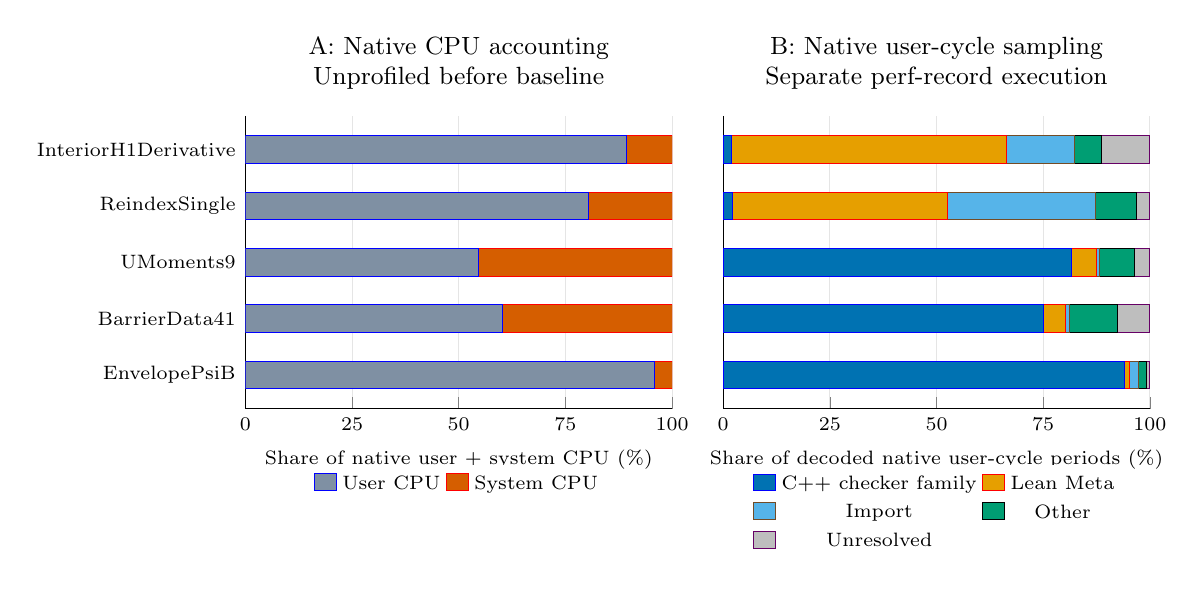
\begin{tikzpicture}
\begin{groupplot}[
group style={group size=2 by 1,horizontal sep=0.65cm},
width=7.0cm,height=5.3cm,
xbar stacked,/pgf/bar width=10pt,xmin=0,xmax=100,
ymin=-0.6,ymax=4.6,y dir=reverse,
ytick={0,1,2,3,4},
xtick={0,25,50,75,100},
tick label style={font=\scriptsize},
title style={font=\small,align=center},
label style={font=\scriptsize},
legend style={font=\scriptsize,draw=none,at={(0.5,-0.19)},anchor=north},
legend columns=2,
axis x line*=bottom,axis y line*=left,
xmajorgrids=true,grid style={gray!20},
every axis plot/.append style={draw=white,line width=0.3pt},
]
\nextgroupplot[
title={A: Native CPU accounting\\Unprofiled before baseline},
yticklabels={InteriorH1Derivative,ReindexSingle,UMoments9,BarrierData41,EnvelopePsiB},
xlabel={Share of native user + system CPU (\%)},
]
\addplot+[fill=cpuuser] coordinates {(89.270754464,0) (80.455578367,1) (54.669456678,2) (60.268848709,3) (95.881593162,4)};
\addplot+[fill=cpusystem] coordinates {(10.729245536,0) (19.544421633,1) (45.330543322,2) (39.731151291,3) (4.118406838,4)};
\legend{User CPU,System CPU}
\nextgroupplot[
title={B: Native user-cycle sampling\\Separate perf-record execution},
yticklabels={,,,,},
xlabel={Share of decoded native user-cycle periods (\%)},
]
\addplot+[fill=checker] coordinates {(1.918358664,0) (2.061032834,1) (81.519978261,2) (74.931485982,3) (94.012196834,4)};
\addplot+[fill=metacolor] coordinates {(64.377219796,0) (50.583787439,1) (5.932139409,2) (5.366720964,3) (1.112226981,4)};
\addplot+[fill=importcolor] coordinates {(16.024740024,0) (34.595452807,1) (0.660601312,2) (0.803501729,3) (2.074184403,4)};
\addplot+[fill=othercolor] coordinates {(6.237972222,0) (9.589319593,1) (8.206964463,2) (11.348307050,3) (2.082983680,4)};
\addplot+[fill=unresolvedcolor] coordinates {(11.441709293,0) (3.170407327,1) (3.680316555,2) (7.549984274,3) (0.718408103,4)};
\legend{C++ checker family,Lean Meta,Import,Other,Unresolved}
\end{groupplot}
\end{tikzpicture}
\end{document}
